\documentclass{article}

\usepackage{neurips_2025_ml4ps}

\usepackage[utf8]{inputenc}
\usepackage[T1]{fontenc}
\usepackage{amsmath,amssymb}
\usepackage{booktabs}
\usepackage{multirow}
\usepackage{multicol}
\usepackage{float}
\usepackage{graphicx}
\usepackage{microtype}
\usepackage[hidelinks]{hyperref}
\usepackage{url}

% Venue-neutral anonymous build: the style file's workshop notice box is
% suppressed so that no venue string appears anywhere in the artifact.
\makeatletter
\renewcommand{\@notice}{}
\makeatother

% Metadata scrub for the double-blind build.
\hypersetup{pdftitle={},pdfauthor={},pdfsubject={},pdfkeywords={},pdfcreator={},pdfproducer={}}

\title{Retention You Can Predict, Scope and Delete:\\ a $(\mu,\gamma,T)$ Law and a Structural Deletion Guarantee\\ for a Physics-Structured Memory Store}

\author{}

\renewcommand{\topfraction}{0.92}
\renewcommand{\bottomfraction}{0.75}
\renewcommand{\textfraction}{0.06}
\renewcommand{\floatpagefraction}{0.85}
\setlength{\textfloatsep}{6pt plus 2pt minus 2pt}
\setlength{\intextsep}{6pt plus 2pt minus 2pt}
\setlength{\abovecaptionskip}{3pt}
% Cosmetic, content-neutral: tighter heading skips so the 4-pp main-text limit is
% met by typography rather than by cutting text.
\makeatletter
\renewcommand\section{\@startsection{section}{1}{\z@}{-1.1ex plus -0.4ex minus -.2ex}{0.7ex plus .2ex}{\normalsize\bf\raggedright}}
\renewcommand\subsection{\@startsection{subsection}{2}{\z@}{-0.9ex plus -0.4ex minus -.2ex}{0.5ex plus .2ex}{\normalsize\bf\raggedright}}
\makeatother
\setlength{\belowcaptionskip}{0pt}
\begin{document}
\maketitle
\begin{abstract}
What a memory system forgets is set by policy: a decay factor, an expiry timestamp, a learned forget gate. Such a policy states when an entry expires, not how fast the stored value degrades, what moving the dial buys, or what remains once it is removed. We answer all three on a physics-structured memory store --- a damped symplectic step of a learned Hamiltonian --- whose retention policy is a budget in three numbers: the stored direction's spectral mass $\mu$, the damping $\gamma$ and the temperature $T$. The dial has a computable optimum: retention half-life is non-monotone in friction, one V-curve minimized at $\gamma_{\rm crit}=2\varepsilon\mu$ ($\propto\mu^{-2}$ overdamped, a mass-independent floor underdamped), spanning $\approx11$ orders of magnitude in $\mu^2$, holding on emergent (learned-MLP) as well as designed units, 3/3 seeds (dim 4, hidden 64, laptop-CPU), and reproduced by direct nonlinear rollout with the argmin agreeing to $0.35\%$. Retention is scopeable: at $T>0$ friction preserves and temperature erases, so a localized friction hole is a memory vault, $107.77\pm4.78\times$ designed and $106.1\pm5.0\times$ law-referenced on emergent (3 seeds each), though the field-versus-scalar contrast naming its mechanism is designed-only. Removal is structural: under canonical placement --- Blelloch \& Golovin's (FOCS'07) --- store-level deletion is exact, the post-deletion store byte-identical at every load measured to the store that never held the item, under three stated conditions (\texttt{budget >= n\_cells}, \texttt{leak = 0}, priority/attribute eviction; recency eviction excluded), on a designed store of dim 3, capacity 8--64, no learning. We state what decay does \emph{not} buy: against an exact adversary a boolean TTL flag in the same store is as detectable as physical decay, and the store stops answering before it stops leaking.
\end{abstract}

\section{Introduction}\label{sec:intro}

Every deployed memory store already runs a retention policy: a decay factor, an invalidation timestamp, a learned forget gate, a \texttt{DELETE} call. Forgetting, however, is the failure mode benchmarks do not measure (Yang, 2026; Uddin et al., 2026), and a policy is not a law. One cannot read off a trained LSTM the half-life of a stored value, the knob that sets it, or what remains once the value is removed. We study a memory whose forgetting is a dynamical property of the store, not a bookkeeping rule over it, so that three operational questions have computable answers: \emph{what is the retention policy, and where is its optimum} (\S\ref{sec:vcurve}); \emph{can retention be scoped to one item} (\S\ref{sec:vault}); \emph{is deletion real, and what still leaks} (\S\ref{sec:deletion}).

Physics enters only as the derivation apparatus. The store's state $(q,p)$ advances by a damped symplectic step of a learnable Hamiltonian $H=T(p)+V_\theta(q)$: the damping $p\mapsto(1-\gamma)p$ supplies forgetting, Langevin noise supplies temperature $T$, and items are optionally written as \emph{atoms}: localized wells superposed into one energy function a dynamical relaxation reads. Our reference unit is the CLU (Causal Learning Unit), introduced as CHLU in Jawahar \& Pierini (2026). Its core is exactly solvable: diagonalised in the mass-whitened Hessian, one damped step acts on each normal mode as a single $2\times2$ matrix fixed by $(\varepsilon\mu,\gamma)$, whose spectral radius is that mode's retention (Anonymous, 2026, a theory note on which nothing here depends).

\paragraph{Contributions.} \emph{(1) A retention dial with a computable optimum} (\S\ref{sec:vcurve}--\S\ref{sec:vault}): retention is non-monotone in the dial and the optimum is predicted, not tuned --- one V-curve minimized at $\gamma_{\rm crit}=2\varepsilon\mu$, so latch, overdamped register and underdamped working memory are three regimes of one curve, evaluated at two values of $\mu$, not two laws, across $\approx11$ decades in $\mu^2$, on emergent as well as designed units, on two instruments. \emph{(2) Scoped retention} (\S\ref{sec:vault}): at $T>0$ friction preserves and temperature erases, so a local change to the dial confines one item's coordinate, and a friction hole is a vault whose two constituent laws hold on both arms. \emph{(3) A structural deletion guarantee} (\S\ref{sec:deletion}), a composition and not a new deletion algorithm: the placement rule and its delete-time repair are Blelloch \& Golovin's (FOCS'07); new here is only the composition --- a lattice packing certificate, decaying content whose decay provably commutes with deletion, one canonical energy function read by a dynamical relaxation --- which makes the store's state a function of its live set alone, plus the trilemma that prices lifetimes and an honest leakage statement. \emph{(4)} A three-state memory lifecycle (PROTECTED $\rightleftarrows$ ACTIVE $\to$ TRASH, 7/7 legs, kill-conditions committed before the verbs, one leg unexercised) --- the consolidation and stale-entry face of the same store --- shipped as a mechanics demonstration on a toy synthetic build: no value or benchmark number is claimed, and none was run.

\emph{What class of claim this is.} Our evidence is a small designed store measured at laptop scale: not a deployed agent memory, not an LLM system, not a benchmark result. We report a mechanism with measured laws, not a system result.

{\scriptsize\emph{Nomenclature, because ``mass'' names two opposed quantities.} The inertial mass $M_i$ is the learned diagonal of the kinetic term (larger $\Rightarrow$ slower); the spectral mass is $\mu_k^2=\lambda_k(M^{-1/2}\nabla^2V_\theta M^{-1/2})$ (larger $\Rightarrow$ shorter memory). Retention statements use $\mu$; a stored value lives on a near-flat coset direction; $\varepsilon$ is the integrator step, $=0.05$, never a tilt. Half-lives mean nothing without a read tolerance $\Delta$ and the thermal persistence length $\ell_\theta$, so we never quote an $n_{1/2}$ without its $\Delta$ and $\ell_\theta/\Delta$, and never read a designed-versus-learned distinction off raw exponents. Results on designed testbeds are labelled verification of exactness; on learned or emergent potentials, evidence. Every $T>0$ result requires the fluctuation--dissipation-consistent noise scale $\sigma^\star_i=\sqrt{M_iT\gamma(2-\gamma)}$ \emph{and} a Newtonian kinetic mode. These laws govern the store; end-to-end performance additionally depends on the encoder, measured separately, $\varphi$-bytes ledgered.\par}

\section{Related work}\label{sec:related}

{\scriptsize\emph{Retention policies in deployed memory systems.} Agent memories are external stores a model writes to, retrieves from and edits (MemGPT, Packer et al., 2023; Mem0, Chhikara et al., 2025), or bounded compressive state inside the network (Infini-attention, Munkhdalai et al., 2024). Their retention policies are scores and gates: a $0.995$ recency decay factor in a ranking heuristic (Generative Agents, Park et al., 2023), an Ebbinghaus decay of memory strength (MemoryBank, Zhong et al., 2024), a learned per-memory expiration span (Expire-Span, Sukhbaatar et al., 2021), and a learned forget gate $\alpha_t$ in $\mathcal M_t=(1-\alpha_t)\mathcal M_{t-1}+S_t$ (Titans, Behrouz et al., 2025) --- the nearest published neighbour to the dial of \S\ref{sec:vcurve}. None states a half-life, a read tolerance or a temperature, and none prices what is lost. We benchmark against none of them; the contrast is structural, our $(\mu,\gamma,T)$ budget occupying the same slot with those three quantities attached.

\emph{Deletion, deployed and formal.} Zep invalidates a contradicted edge with a timestamp and preserves the record (Rasmussen et al., 2025); Mem0's DELETE removes a row. Byte-identity is the opposite design point, and it matters because soft-deleted vectors stay reconstructible from raw index files in graph ANN databases (Chakraborttii et al., 2026). A 2026 evaluation wave motivates the framing: production failures are predominantly forgetting failures while benchmarks measure recall (Yang, 2026), failures to forget outdated memory drive a large share of sampled recommendation errors (Uddin et al., 2026), deleted facts stay recoverable through retained correlated modalities (Wang \& Zhang, 2026), and agentic unlearning must handle reactivation out of persistent memory (Wang et al., 2026) --- the last two being why \S\ref{sec:deletion}'s encoder-excluded scope is a scope, not a hedge: the store deleting an item is not the system forgetting it. Formally, \emph{certified} removal is Guo et al.'s (2020) \S2 Eq.~(1), an $\varepsilon$ condition with an unnumbered $(\varepsilon,\delta)$ relaxation immediately after; exact methods delete by isolation, with cost and capacity formalisms in place (Bourtoule et al., 2021; Ginart et al., 2019; Sekhari et al., 2021). We make none of those claims: ours is a store-level bit-exactness statement with the encoder excluded, coining no benchmark and no cost claim. Order-independent placement is not ours either --- Snyder (1977) through Naor \& Teague (2001) to Blelloch \& Golovin (2007), whose table we use; and Blelloch, Golovin \& Vassilevska (2008) had already taken unique representation into computational geometry, so canonical placement in a geometric setting is not virgin ground (Appendix~\ref{app:deletion}).

\emph{Forgetting laws, learned and physical.} Learned recurrent comparators (LSTM, Hochreiter \& Schmidhuber, 1997; LEM, Rusch et al., 2022) lack a stateable forgetting law. In physics, dissipation turns type-A Nambu--Goldstone modes from propagating to diffusive (Minami \& Hidaka, 2018) --- exactly our coset --- and Mo (2026) proves that an exactly $G$-equivariant flow has \emph{at least} $\dim(G/\mathcal H)$ zero Lyapunov exponents along the orbit: the kinematics of protection, to which our budget is the constitutive complement, since the gap is $\mu^2$.\par}

\section{Results}\label{sec:results}

\subsection{The retention dial has a computable optimum}\label{sec:vcurve}

If damping is the retention dial, where should it be set? Not by tuning, and not at the low end: retention half-life is non-monotone in friction, and the turning point is fixed by the stored direction's spectral mass, so the optimum is predicted.

The step is conformally symplectic, $\det J=(1-\gamma)^d$, and $(1-\gamma\phi(q'))^d$ when position-gated; checkpoints (dim 4, hidden 64, $\varepsilon=0.05$, 150 epochs) are \emph{designed} ($SO(2)$-invariant $V_\theta$, 5 seeds) or \emph{emergent} (MLP $V_\theta$ on identical symmetric data, 3 seeds). On a trained designed-$SO(2)$ vacuum the massive radial mode's $n_{1/2}(\gamma)$ is a V minimized at $\gamma_{\rm crit}=2\varepsilon\mu_{\rm rad}$, the overdamped branch following the $\mu^{-2}$ law up to $\varepsilon\mu\approx\gamma/2$ and then saturating at a mass-independent floor (log-slopes $-1.006$ and $+1.23$--$+1.27$; 5 seeds, verification, Appendix~\ref{app:budget}). The flat coset (Hessian $\mu^2\approx10^{-15}$) is the \emph{same curve at $\mu\to0$}, where $\gamma_{\rm crit}\to0$: latch, overdamped register and underdamped working memory are three regimes of one curve, evaluated at two values of $\mu$ --- not two laws. It generalizes to emergent units (evidence): on three emergent MLP checkpoints trained on the same symmetric data the coset-tracked $T=0$ half-life traces the same V-curve --- argmin $0.902\pm0.003\times\gamma_{\rm crit}$, log-slopes $-1.0020\pm0.0003$ / $+1.116\pm0.011$, 3/3 seeds. Across both families the curve spans $\mu^2\in[1.7\times10^{-12},\,7\times10^{-2}]$, that low endpoint being the ring-profile probe's resolution on a checkpoint whose Hessian $\mu^2$ is machine zero rather than a spectral mass --- so eleven orders is one curve on one instrument, though the $\mu\to0$ corner has its own model-side bound of $n_{1/2}\ge9.5\times10^{15}$ steps by direct $T=0$ rollout (Appendix~\ref{app:emergent}).
\begin{figure}[t]
\centering
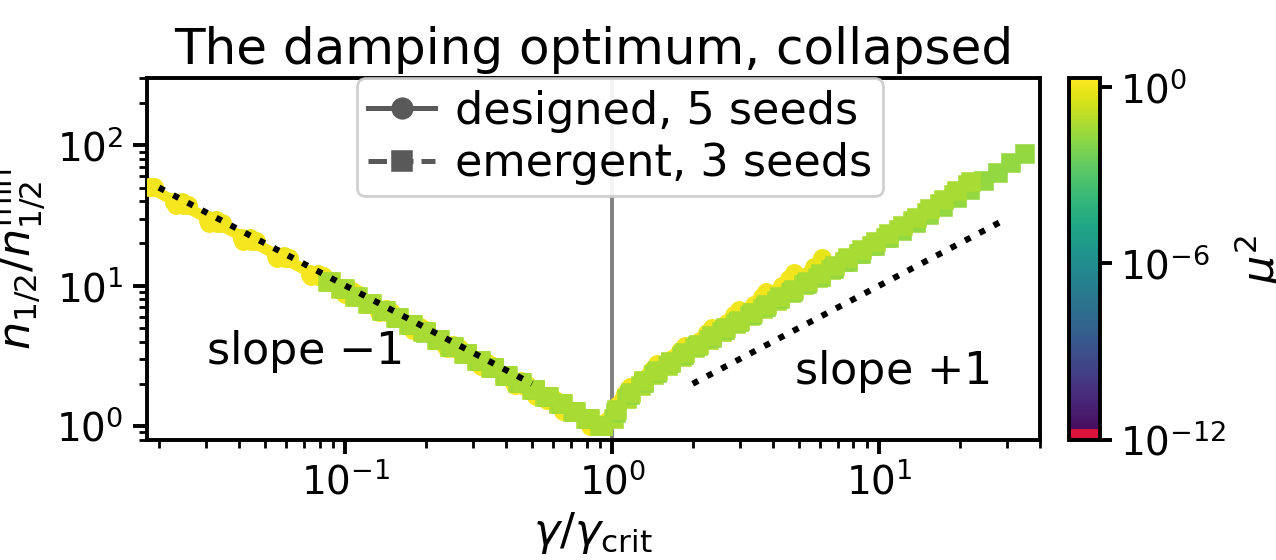
\includegraphics[width=0.58\linewidth]{figs/fig1_damping_optimum.png}
\caption{\emph{The retention dial and its optimum, collapsed (headline).} Eight measured curves collapse onto one: five designed radial modes (circles, verification, $\mu^2_{\rm rad}=0.670$--$1.348$) and three emergent learned-MLP coset modes (squares, evidence, $\mu^2_{\rm soft}=2.0$--$5.4\times10^{-2}$, 3/3 seeds), against the $\mp1$ asymptotes; the designed flat coset is the $\mu\to0$ corner of the same curve. \emph{(One-step Jacobian; dim 4, hidden 64, $\varepsilon=0.05$, laptop-CPU; \texttt{langevin\_noise="fdt"}, Newtonian kinetic mode.)}}
\label{fig:collapse}
\end{figure}

\emph{Two instruments, one law (evidence).} Every point above is a one-step Jacobian, so we re-measured the curve by direct nonlinear rollout, reading $n_{1/2}$ from the decay envelope's rate (3 emergent seeds, $\delta=0.05$--$0.5$ rad). The shape reproduces: argmin $0.9001\pm0.0052$ against the Jacobian's $0.9032\pm0.0027$ in units of $\gamma_{\rm crit}$ --- a $0.35\%$ difference --- log-slopes $-0.983\pm0.013$ / $+1.117\pm0.010$ on identical fit windows, and decay \emph{rates} agreeing to $0.995\pm0.003$ in the asymptotic window. The instruments differ by a level, not a law: a first-crossing threshold reads short by a per-checkpoint constant ($1.33$/$1.80$/$1.82\times$) flat in $\gamma$, with coefficient of variation $2.2$--$3.7\%$. {\scriptsize\emph{What would have falsified the law:} a stored direction that mixes normal modes, or is anharmonic at the write amplitude, has no single-mode reduction, so the curves would neither collapse nor put their minimum at $2\varepsilon\mu$; neither happens at ten times the write amplitude, where the argmin moves by at most $1.4\%$ (to $0.897$--$0.917\,\gamma_{\rm crit}$) and the slopes by at most $1.9\%$ (Appendix~\ref{app:emergent}).\par}

\subsection{Scoping retention to one item: friction preserves, temperature erases}\label{sec:vault}

Scoping a policy to one entry means changing the dial locally, and the sign of the dial's effect on a stored value is not the expected one. At $T=0$ a designed coset latches forever at any friction (drift $\le4.9\times10^{-12}$ rad over $200$k steps, all $\gamma\in[0.002,0.5]$, 5 seeds, verification): friction has no contractive action on a flat direction. At $T>0$ the coset decays diffusively and friction slows it down --- $D_\theta=\varepsilon T(2-\gamma)/(2F^2\gamma)$ is verified to $1.0068\pm0.0219$ over 25 $(\gamma,T)$ cells, so $n_{1/2}\propto\gamma^{+1}$ and the sign flip $\partial n_{1/2}/\partial\gamma>0$ holds in 10/10 seed $\times$ temperature conditions, $\gamma:0.05\to0.2$ \emph{lengthening} the half-life $3.77\pm0.23\times$ at $\Delta=0.5$ rad, $\ell_\theta/\Delta<0.05$; only temperature has $\partial n_{1/2}/\partial T<0$. {\scriptsize\emph{Fine print, beside the claim:} every $T>0$ number requires \texttt{langevin\_noise="fdt"} \emph{and} a Newtonian kinetic mode; under the reference default these laws fail, and in the relativistic mode no noise scale targets Gibbs.\par}

\emph{Hence a memory vault.} The shipped position-gated friction field is \emph{absorb-only}, so a hole is a brake \emph{and} a refrigerator ($T_{\rm local}=1.26\times10^{-4}$ against $10^{-3}$ outside, where a coupled bath predicts none), and the vault factor is $(\gamma_{\rm eff}/\gamma)^2$ --- $107.77\pm4.78\times$ ($D_\theta$-estimator, pre-registered, 3 designed seeds, $\Delta=0.5$ rad) against $13.28\pm0.12\times$ for a scalar friction of equal $\gamma_{\rm eff}$, the ratio $8.11\pm0.37$ being the refrigerator. At $T=0$ it erases nothing. Both laws transfer to an emergent register (evidence, 3 emergent seeds at $T=4\times10^{-3}$ and $8\times10^{-3}$, both above $T^\star$): the refrigerator law holds at $0.9998\pm0.0019$ of prediction (the coupled bath rejected again at $0.2235$) and the $\hat D_\theta\propto\gamma_{\rm eff}^{-2}$ law at $1.016$--$1.103$, a law-referenced vault of $106.1\pm5.0\times$ beside the designed $107.77\pm4.78\times$. One result has no designed analogue, and it is the one that makes scoping operational --- \emph{the hole confines}: the fraction of states outside the register ($|\theta|>1$ rad) falls from $5.5/43.0/2.4\%$ with no hole to $0.0000$ inside it, 3/3 seeds, while a scalar friction of the same $\gamma_{\rm eff}$ still hops ($0.73/10.2/0.26\%$). {\scriptsize\emph{The contrast number stays designed-only:} on emergent the field/scalar ratio measures $23.39\pm10.06$ because the \emph{control} arm delocalises there ($\hat D/D_{\rm flat}=1.18$--$5.23$) while the field arm sits on the law, so $8.11\pm0.37$ is a designed quantity and the direction, not the number, transfers. We quote no emergent $\sigma_\theta$ ratio: above $T^\star$ that diagnostic is non-stationary here, its control returning $0.459\pm0.118$ where it must return $1.000$ (Appendix~\ref{app:vault}).\par} \emph{The designed-symmetry precondition, the boundary on everything above} (evidence; 3 emergent seeds and a matched designed control). The exact $T=0$ latch is a \emph{designed} object: on an MLP potential trained on identical symmetric data the softest direction is a mid-spectrum massive mode ($1-|\lambda_{\rm coset}|\approx10^{-3}$ against the designed $\le1.1\times10^{-15}$), a written value relaxes completely, and capacity is $\approx1$--$1.6$ bits. An emergent unit of this class has no continuous coset register, and continuum flat directions must be designed in. What survives is exactly the headline --- the V-curve on 3/3 seeds and the sign flip above a measured $T^\star\approx3\times10^{-3}$. The same boundary bounds an extrapolation we do not make, and Appendix~\ref{app:negatives} records it.

\subsection{Deletion: a structural guarantee, priced lifetimes, and what still leaks}\label{sec:deletion}

\emph{(Designed atom store, dim 3, no learning anywhere $\Rightarrow$ verification.)} Deletion in a deployed store is best-effort: a row dropped, an edge timestamped, a tombstone written. We ask instead whether the store's state can be made a function of its live set alone. Stated once: external benchmarks won on their own headline metric = ZERO. A flat table deletes exactly by construction --- the trivial substitute; at issue is a store whose items are \emph{superposed into one energy function}, where placement would ordinarily depend on which others are present. Placement here is canonical, a function of the live records and the geometry alone, so removal reproduces the store holding the rest bit for bit. Measured: \emph{``with the waitlist, store-level deletion is exact at every load measured, $0.29\times$--$1.71\times$ lattice capacity --- AUC $0.5000\pm0.0000$ on all six statistics, byte-equal $1.0000$ --- under three stated conditions (\texttt{budget >= n\_cells}, \texttt{leak = 0}, priority/attribute-based eviction; recency-based eviction remains intrinsically history-dependent and is excluded).''} The allocator it replaces leaks membership after eviction (AUC $0.99985$ at full load), and the packing price of exactness is negative: canonical placement admits strictly more keys than refuse-and-relocate. {\scriptsize This is a store-level guarantee only --- the frozen encoder and any residue of past writes in a learned landscape are separate channels, measured separately, and we claim no certified $(\varepsilon,\delta)$ unlearning; without the waitlist, exactness fails at overflow (Appendix~\ref{app:deletion}).\par} \emph{Attribution, in the same breath as the theorems.} \emph{Our placement rule is the Blelloch--Golovin (FOCS'07) stable-matching table, our Theorems 1--2 follow from theirs, and the fix-up cascade is theirs.} The composition's price is negative where the general case can cost an exponential slowdown (Buchbinder \& Petrank, 2003). {\scriptsize That separation is between the \emph{weak and strong} notions for comparison-based structures, whereas ours is against a history-\emph{dependent} stochastic relocation rule, so the two statements are adjacent rather than identical.\par} \emph{Lifetimes are priced by a trilemma} --- exact value fidelity, amplitude-independent address hold, amplitude-independent read latency: pick two. The corner to lead with: \emph{dropping amplitude-independent latency} \emph{is} \emph{the compute-adaptive-read dial --- a faded memory costs more integration steps to read, a physical, measurable statement a timestamped row cannot make.}

\emph{What decay does not buy.} The tighter laundering control is the policy already deployed elsewhere, a boolean TTL flag \emph{inside the same store}, and it fires: against an exact adversary the TTL flag stays within $0.017$ AUC of physical decay ($0.983$ versus $1.000$), the two separating only against a resolution-limited adversary ($0.559$ versus $0.996$ at $\sigma_{\rm obs}=0.1$), whose resolution is our own modelling choice. \emph{The store stops answering before it stops leaking}: at the last amplitude before self-eviction ($A=0.051$) retention is $0.832$ --- placement-dependent, quoted for the controller-placed disk --- while a query-level membership adversary sits at AUC $0.983$ and a white-box one at $1.000$; the curves never cross. Against an \emph{exact} adversary decay reduces the effect size, not the AUC, so we claim no reduction in distinguishability per se. What physical decay buys over a TTL flag is retrieval geometry, not privacy, and that differentiator needs no adversary model: \emph{decay contracts the addressing tolerance of an item, $R_{50}$ $1.146\to0.752$ ($1.52\times$), where a TTL dict's lookup radius is a constant hard step at $0.75$--$0.77$, independent of age.}

\section{Limitations and future work}\label{sec:limits}

{\scriptsize\emph{Limitations.} (i) One architecture, one scale: dim 4, hidden 64, laptop-CPU, 5 designed / 3 emergent seeds; store at dim 3, no learning; lifecycle on a toy synthetic build. (ii) The designed-symmetry precondition (\S\ref{sec:vault}). (iii) Raw $T/\gamma$-exponents do not discriminate designed from emergent; the \texttt{fdt} + Newtonian scope is mandatory at every $T>0$. (iv) The V-curve's shape is instrument-independent, its absolute step counts are not (a first-crossing threshold reads $1.33$--$1.82\times$ short of the Jacobian, a constant per-checkpoint offset), and the emergent collapse spans only $2.7\times$ in $\mu^2$ across three seeds, so the eleven decades are one decade of emergent variation attached to the designed $\mu\to0$ corner. (v) Deletion is store-level only, under set-function eviction with recency eviction excluded, and no deletion-cost claim is made ($O(n)$ rebuild per operation; unrun). (vi) No task-level payoff is claimed. \emph{Scale is a scope choice:} this short is sealed to laptop-scale evidence; no larger-scale result is quoted or should be inferred. \emph{Named next:} a wider emergent collapse in $\mu^2$; the vault's contrast arm re-measured where both arms stay bounded; amortized per-delete cost against the flat-datastore substitute; deletion at $10^3$-item stores; and a localized \emph{temperature} field.\par}
\clearpage
\appendix
\scriptsize

\section*{References}
{\tiny\setlength{\columnsep}{14pt}\begin{multicols}{2}\begin{itemize}\itemsep0pt \parskip0pt \leftmargin0pt
\item Andersson, A., \& Ottmann, T. (1995). New tight bounds on uniquely represented dictionaries. \emph{SIAM Journal on Computing} 24(5):1091--1103.
\item Anonymous (2026). \emph{The theory note} (exactly-solvable damped-symplectic retention theory). Anonymized for double-blind review.
\item Behrouz, A., Zhong, P., \& Mirrokni, V. (2025). Titans: Learning to memorize at test time. \emph{NeurIPS 2025}. arXiv:2501.00663.
\item Blelloch, G. E., \& Golovin, D. (2007). Strongly history-independent hashing with applications. \emph{48th IEEE Symposium on Foundations of Computer Science (FOCS)}, 272--282. doi:10.1109/FOCS.2007.36.
\item Blelloch, G. E., Golovin, D., \& Vassilevska, V. (2008). Uniquely represented data structures for computational geometry. \emph{11th Scandinavian Workshop on Algorithm Theory (SWAT)}, LNCS 5124:17--28. doi:10.1007/978-3-540-69903-3\_4.
\item Bourtoule, L., Chandrasekaran, V., Choquette-Choo, C. A., Jia, H., Travers, A., Zhang, B., Lie, D., \& Papernot, N. (2021). Machine unlearning. \emph{42nd IEEE Symposium on Security and Privacy}. arXiv:1912.03817.
\item Buchbinder, N., \& Petrank, E. (2003). Lower and upper bounds on obtaining history independence. \emph{CRYPTO 2003}, LNCS 2729:445--462. Journal version: \emph{Information and Computation} 204(2):291--337 (2006).
\item Chakraborttii, C., Garc\'ia Alvarado, J., Abdulofizova, S., \& Dwivedi, S. (2026). Ghost vectors: Soft-deleted embeddings remain reconstructible in HNSW vector databases. arXiv:2606.18497 (preprint).
\item Chhikara, P., Khant, D., Aryan, S., Singh, T., \& Yadav, D. (2025). Mem0: Building production-ready AI agents with scalable long-term memory. arXiv:2504.19413 (preprint).
\item Ginart, A., Guan, M. Y., Valiant, G., \& Zou, J. (2019). Making AI forget you: Data deletion in machine learning. \emph{NeurIPS 2019}. arXiv:1907.05012.
\item Guo, C., Goldstein, T., Hannun, A., \& van der Maaten, L. (2020). Certified data removal from machine learning models. \emph{ICML}, PMLR 119:3832--3842. arXiv:1911.03030.
\item Hochreiter, S., \& Schmidhuber, J. (1997). Long short-term memory. \emph{Neural Computation} 9(8):1735--1780. doi:10.1162/neco.1997.9.8.1735.
\item Jawahar, P., \& Pierini, M. (2026). \emph{Causal Hamiltonian Learning Units (CHLU)}. [Reference redacted for double-blind review.]
\item Micciancio, D. (1997). Oblivious data structures: Applications to cryptography. \emph{29th ACM Symposium on Theory of Computing (STOC)}, 456--464. doi:10.1145/258533.258638.
\item Minami, Y., \& Hidaka, Y. (2018). Spontaneous symmetry breaking and Nambu--Goldstone modes in dissipative systems. \emph{Physical Review E} 97(1):012130. doi:10.1103/PhysRevE.97.012130.
\item Mo, H. H. (2026). Symmetry-protected Lyapunov neutral modes in equivariant recurrent networks. arXiv:2605.03338 (preprint; single author).
\item Munkhdalai, T., Faruqui, M., \& Gopal, S. (2024). Leave no context behind: Efficient infinite context transformers with Infini-attention. arXiv:2404.07143 (preprint).
\item Naor, M., \& Teague, V. (2001). Anti-persistence: History independent data structures. \emph{33rd ACM Symposium on Theory of Computing (STOC)}, 492--501. doi:10.1145/380752.380844.
\item Packer, C., Wooders, S., Lin, K., Fang, V., Patil, S. G., Stoica, I., \& Gonzalez, J. E. (2023). MemGPT: Towards LLMs as operating systems. arXiv:2310.08560 (preprint).
\item Park, J. S., O'Brien, J. C., Cai, C. J., Morris, M. R., Liang, P., \& Bernstein, M. S. (2023). Generative agents: Interactive simulacra of human behavior. \emph{UIST 2023}. arXiv:2304.03442.
\item Rasmussen, P., Paliychuk, P., Beauvais, T., Ryan, J., \& Chalef, D. (2025). Zep: A temporal knowledge graph architecture for agent memory. arXiv:2501.13956 (preprint).
\item Rusch, T. K., Mishra, S., Erichson, N. B., \& Mahoney, M. W. (2022). Long expressive memory for sequence modeling. \emph{ICLR 2022}. arXiv:2110.04744.
\item Sekhari, A., Acharya, J., Kamath, G., \& Suresh, A. T. (2021). Remember what you want to forget: Algorithms for machine unlearning. \emph{NeurIPS 2021}, 18075--18086. arXiv:2103.03279.
\item Snyder, L. (1977). On uniquely representable data structures. \emph{18th IEEE Symposium on Foundations of Computer Science (FOCS)}, 142--146.
\item Sukhbaatar, S., Ju, D., Poff, S., Roller, S., Szlam, A., Weston, J., \& Fan, A. (2021). Not all memories are created equal: Learning to forget by expiring. \emph{ICML 2021}. arXiv:2105.06548.
\item Uddin, M. N., Shubham, K., Blanco, E., Baral, C., \& Wang, G. (2026). From recall to forgetting: Benchmarking long-term memory for personalized agents. arXiv:2604.20006 (preprint).
\item Wang, B., Wang, F., Wang, P., Cong, J., Yu, Y., Yin, Y., Han, Z., \& Wei, B. (2026). Agentic unlearning: When LLM agent meets machine unlearning. arXiv:2602.17692 (preprint).
\item Wang, K., \& Zhang, C. (2026). MemLeak: Diagnosing information leaks in multimodal agent memory. arXiv:2606.29788 (preprint).
\item Yang, D. (2026). Control-plane placement shapes forgetting: An architectural study of agent memory across thirteen system configurations. arXiv:2606.15903 (preprint).
\item Zhong, W., Guo, L., Gao, Q., Ye, H., \& Wang, Y. (2024). MemoryBank: Enhancing large language models with long-term memory. \emph{AAAI 2024}. arXiv:2305.10250.
\end{itemize}\end{multicols}\par}
\section{The $(\mu,\gamma,T)$ budget: the diffusion law and the sign flip}\label{app:budget}

\emph{Designed $SO(2)$ testbed $\Rightarrow$ verification. All $T>0$ cells require \texttt{langevin\_noise="fdt"} and a Newtonian kinetic mode; the reference default is \texttt{legacy}, under which none of these laws hold. Every $n_{1/2}$ is quoted with its read tolerance $\Delta=0.5$ rad and its $\ell_\theta/\Delta$.}

\emph{Diffusion law, 25 cells} ($5\gamma\times5T$, seed 44): $\hat D_\theta/D_\theta^{\rm pred}=1.0068\pm0.0219$ (min $0.9644$, max $1.0484$); $d\log D/d\log T=+0.998,+0.997,+0.992,+1.010,+1.006$; $d\log D/d\log\gamma=-1.014,-0.980,-0.999,-1.001,-0.982$ after dividing the discrete $(2-\gamma)$ factor. \emph{Sign flip:} $d\log n_{1/2}/d\log\gamma=+0.9552\pm0.0422$ at $T=10^{-3}$, 5 seeds, positive in 10/10 conditions; effect size $\gamma:0.05\to0.2$ is $3.77\pm0.23\times$ (per-seed $3.55,3.64,3.61,3.89,4.15$); $d\log n_{1/2}/d\log T=-0.956$ to $-0.979$ deep-diffusive. \emph{Latch at $T=0$, designed only:} $\big||\lambda_{\rm flat}|-1\big|\le1.7\times10^{-14}$ over 22 $\gamma$ values on 5 seeds, drift $\le4.9\times10^{-12}$ rad per 200k steps in 30/30 cells, against a $\gamma=0$ control drifting $142.7$ rad per 20k. \emph{Designed V-curve:} argmin $0.076$--$0.096$ against a predicted $0.082$--$0.116$ (per-seed $\mu^2_{\rm rad}=0.670,0.771,1.190,1.093,1.348$); asymptotic log-slopes $-1.006$ and $+1.23$--$+1.27$; mass-independent floor $27.03$ steps at $\gamma=0.05$.

\begin{table}[!htb]\centering\scriptsize
\caption{The $T>0$ face of the budget, all four entries measured on the designed testbed.}
\begin{tabular}{lll}
\toprule
stored direction & $\partial n_{1/2}/\partial\gamma$ (more friction) & $\partial n_{1/2}/\partial T$ (more heat)\\
\midrule
coset / flat (designed) & $>0$, friction \emph{preserves} ($+0.955\pm0.042$; $3.77\times$ for $\gamma:0.05\to0.2$) & $<0$, temperature \emph{erases} ($-0.956$ to $-0.979$)\\
massive (underdamped) & $<0$, friction shortens (slope $-1.006$) & $\approx0$; $T$ sets only the fluctuation floor (max/min $\le1.013$, 9/9)\\
\bottomrule
\end{tabular}
\end{table}

\section{The emergent arm, and the V-curve on a second instrument}\label{app:emergent}
\begin{figure}[!htb]
\centering
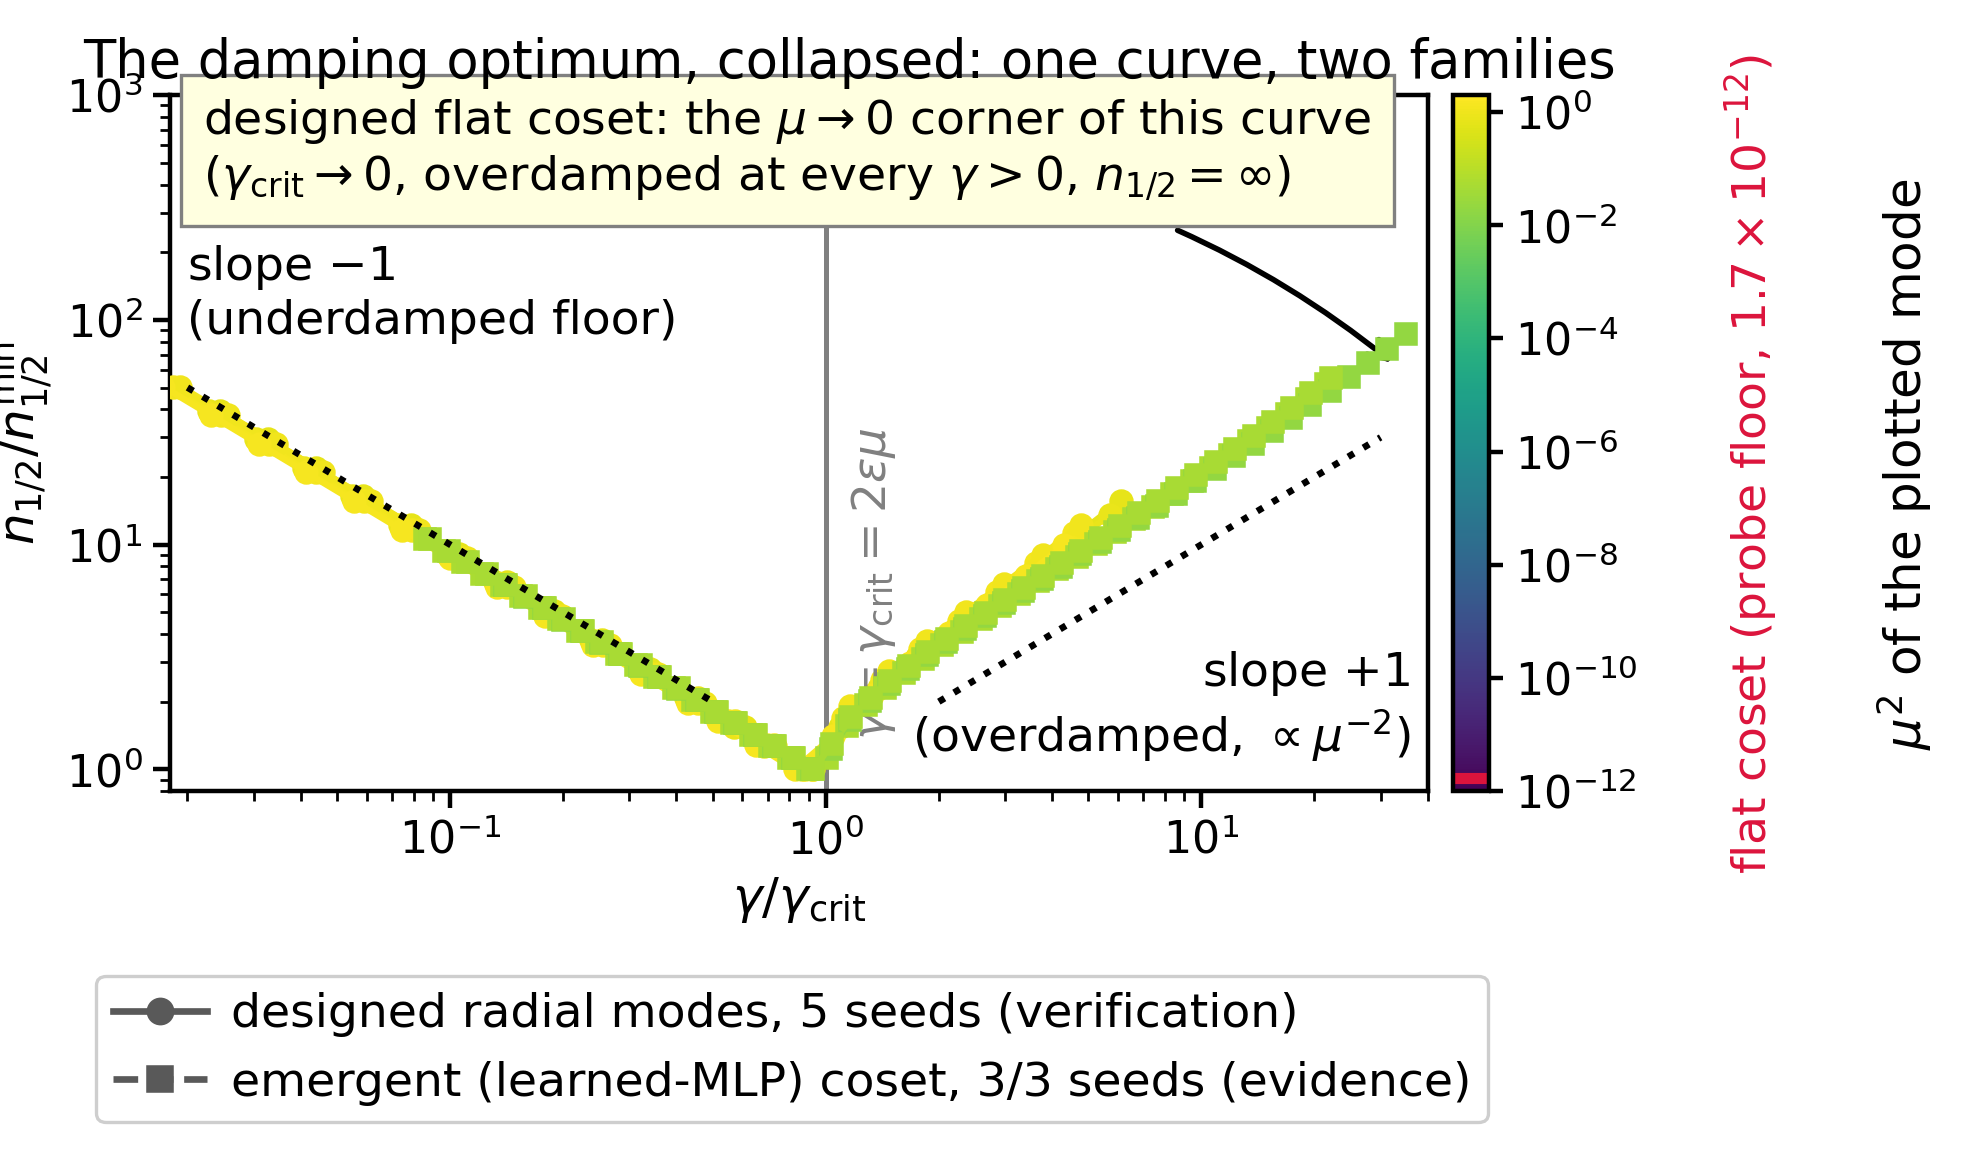
\includegraphics[width=0.90\linewidth]{figs/figA1_damping_optimum_full.png}
\caption{\emph{The damping optimum, collapsed --- the full-size version of Figure~\ref{fig:collapse}.} The same eight measured curves and the same $\mp1$ asymptotes, printed large enough to carry the annotations the main-text box cannot hold: the two-family legend, the $\gamma=\gamma_{\rm crit}=2\varepsilon\mu$ marker, the $\mu\to0$ flat-coset callout, and the crimson probe-floor tick on the $\mu^2$ colourbar ($1.7\times10^{-12}$). No plotted value differs from Figure~\ref{fig:collapse}. \emph{(One-step Jacobian; dim 4, hidden 64, $\varepsilon=0.05$, laptop-CPU; \texttt{langevin\_noise="fdt"}, Newtonian kinetic mode.)}}
\label{fig:collapse-full}
\end{figure}


\emph{Emergent MLP checkpoints, 3 seeds, plus a matched designed control $\Rightarrow$ evidence. Pre-registered; predictions filed before any harness ran.}

\emph{Four instruments, identical fit windows} ($\gamma<\gamma_{\rm crit}/2.5$, $\gamma>2.5\gamma_{\rm crit}$, keyed to the Jacobian's $\gamma_{\rm crit}$ so the windows are not a free parameter): \emph{I-J}, the one-step Jacobian, $n_{1/2}=\ln2/(-\ln|\lambda_{\rm ret}|)$; \emph{I-R1}, rollout first crossing of $|\theta|\le\delta/2$; \emph{I-R2}, rollout last crossing; \emph{I-R3} (primary), rollout envelope-rate fit over the late window, $R^2\ge0.9955$ (median $0.9996$) on every cell.

\begin{table}[!htb]\centering\scriptsize
\tiny\caption{The shape claims on all four instruments ($\delta=0.05$ rad, 48 $\gamma$ values, 3 emergent seeds). The rollout rate instrument reproduces the Jacobian; both threshold instruments fail below $\gamma_{\rm crit}$, so no rollout $n_{1/2}$ is ever quoted from a threshold there.}
\begin{tabular}{lcccc}
\toprule
 & $\gamma_{\rm crit}$ & argmin$/\gamma_{\rm crit}$ (I-J / I-R1 / I-R2 / I-R3) & slope below & slope above\\
\midrule
seed 42 & $0.02334$ & $0.8994$ / $0.0857$ / $0.2068$ / $0.8928$ & $-1.0023$ / $+0.0725$ / $-1.0556$ / $-0.9651$ & $+1.1262$ / $+1.1027$ / $+1.1027$ / $+1.1255$\\
seed 43 & $0.01424$ & $0.9046$ / $0.1404$ / $0.1404$ / $0.9047$ & $-1.0016$ / $+0.0688$ / $+0.0688$ / $-0.9977$ & $+1.1031$ / $+1.0889$ / $+1.0889$ / $+1.1030$\\
seed 44 & $0.02265$ & $0.9055$ / $0.0883$ / $0.3031$ / $0.9028$ & $-1.0022$ / $+0.0455$ / $-0.8854$ / $-0.9854$ & $+1.1254$ / $+1.0977$ / $+1.0977$ / $+1.1231$\\
\midrule
mean $\pm$ sd & & $0.9032\pm0.0027$ / $0.1048\pm0.0252$ / $0.2168\pm0.0668$ / $0.9001\pm0.0052$ & $-1.0020\pm0.0003$ / $+0.0623\pm0.0120$ / $-0.6240\pm0.4948$ / $-0.9827\pm0.0134$ & $+1.1182\pm0.0107$ / $+1.0964\pm0.0057$ / $+1.0964\pm0.0057$ / $+1.1172\pm0.0101$\\
\bottomrule
\end{tabular}
\end{table}

\begin{table}[!htb]\centering\scriptsize
\tiny\caption{The instrument gap is a level, not a rate: on the overdamped branch ($\gamma\ge2\gamma_{\rm crit}$) the decay \emph{rates} agree while the \emph{threshold} instrument is offset by a per-checkpoint constant flat in $\gamma$. Seed 44's full-window value ($0.9216\pm0.0027$) sits $0.0004$ below its pre-registered band because that window still contains a second, faster mode (early-window ratio $0.539$); the window-split diagnostic converges monotonically to $1$ into the asymptote. Cause of the threshold offset, measured: the ring write deposits only a fraction of its amplitude in the slow branch (envelope-fit intercept over $\delta$ = $0.638/0.644/0.327$).}
\begin{tabular}{lccc}
\toprule
seed & $\Gamma_{\rm jac}/\Gamma_{\rm R3}$ (asymptotic window) & $n_{\rm jac}/n_{\rm R1}$ (threshold) & CV of $n_{\rm jac}/n_{\rm R1}$ over the grid\\
\midrule
42 & $0.9935$ & $1.3307$ & \multirow{3}{*}{$2.2$--$3.7\%$ over 21--25 $\gamma$-points}\\
43 & $1.0000$ & $1.7981$ & \\
44 & $0.9948$ & $1.8204$ & \\
\midrule
mean & $0.995\pm0.003$ & per seed, at $\delta=0.05$ rad & $|d\log(\text{ratio})/d\log\gamma|\le0.0034$ (threshold $0.10$)\\
\bottomrule
\end{tabular}
\end{table}

\emph{Finite write amplitude.} At $\delta=0.05/0.2/0.5$ rad the I-R3 argmin is $0.8928/0.9007/0.8968$ (seed 42), $0.9047/0.9045/0.9174$ (43), $0.9028/0.9037/0.9070$ (44) --- at most $+1.4\%$ over a $10\times$ range --- and the slopes move by at most $1.9\%$; every $\delta=0.5$ write relaxed all the way home ($|\theta_{\rm final}|\le6.5\times10^{-10}$), so no seed's write cleared its washboard barrier. The pre-registered early-window clause \emph{fails}, $\Gamma_{\rm jac}/\Gamma^{\rm early}_{\rm roll}=0.52$--$0.85$ against a band of $[0.65,1.35]$; the amplitude sweep identifies that as mode mixing rather than anharmonicity, seed 44's early ratio being $0.539/0.527/0.522$ across the same $10\times$ range.

\emph{What the left branch does not contain.} For $\gamma<\gamma_{\rm crit}$ the coset eigenpair is complex with $|\lambda|^2=1-\gamma$, so $n_{1/2}=\ln2/(-\tfrac12\ln(1-\gamma))$ \emph{independently of $\mu^2$ and of the checkpoint}: at $\gamma=0.002$, emergent seeds 42 ($\mu^2=5.449\times10^{-2}$) and 43 ($\mu^2=2.029\times10^{-2}$) both print $\lambda_{\rm ret}=0.998999499$ and $n_{1/2}=692.5$, against $2\ln2/0.002=693.1$. All model-dependent content of the V-curve is the argmin location $\gamma_{\rm crit}=2\varepsilon\mu$ and the $+1$ branch; what the rollout adds is that the \emph{nonlinear} model obeys that identity, which was not guaranteed.

\emph{Designed control, and the model-side bound.} Over 5 designed seeds $\times$ 48 $\gamma$ $\times$ 3 write amplitudes $\times$ 32\,000 steps of direct $T=0$ rollout, $\max_n|\theta(n)-\delta|=9.400\times10^{-13}$ rad, so $\Gamma\le7.309\times10^{-17}$ per step and $n_{1/2}\ge9.483\times10^{15}$ steps against a pre-registered bound of $10^{-6}$ rad; the matched Hessian $\mu^2_{\rm soft}$ there is $1.60\times10^{-15}$, $1.52\times10^{-15}$, $-2.92\times10^{-16}$, $2.94\times10^{-16}$, $1.21\times10^{-16}$. \emph{Collapse:} in $x=\gamma/\gamma_{\rm crit}$, $y=n_{1/2}\gamma_{\rm crit}$ the three emergent curves agree to a median $1.15\%$ on I-J and $5.67\%$ on I-R3; $y_{\min}=1.579/1.527/1.499$ and $1.631/1.535/1.662$ sit $22$--$24\%$ below the continuum $2\sqrt2\ln2=1.961$ and $x_{\min}\approx0.90$ sits $27\%$ above the continuum $0.707$, both known discrete-map corrections (matched designed control $x_{\min}=0.83$--$0.93$). \emph{Scope:} $\mu^2_{\rm soft}$ spans only $2.029\times10^{-2}$--$5.449\times10^{-2}$ across the three seeds, a factor $2.7$, so the eleven-decade span is one decade of emergent variation attached to the designed $\mu\to0$ corner and the rollout does not widen it.

\emph{The emergent arm's own negative.} $1-|\lambda_{\rm coset}|=1.06\times10^{-3}$--$2.96\times10^{-3}$ at $\gamma\approx0.048$ against a designed $\le1.1\times10^{-15}$, with a whole-grid emergent minimum of $7.6\times10^{-5}$--$2.0\times10^{-4}$ against a designed grid minimum of exactly $0$. Written $\delta\in\{0.1,0.3,0.5\}$ rad relaxes completely ($|\text{retained}|\le2.1\times10^{-3}$) where the designed checkpoint retains $\delta$ exactly; capacity is $\approx1$--$1.6$ bits, not a continuum. Bias-corrected $n_{1/2}^{\rm obs}/n_{1/2}^{\rm Goldstone}$ at $\gamma=0.2$, $\ell_\theta/\Delta<0.06$, runs $2.75, 3.40$ at $T=2\times10^{-3}$ to $0.94$--$1.25$ at $T\ge4\times10^{-3}$, giving $T^\star\approx3\times10^{-3}$ (predicted $2.72$--$3.66\times10^{-3}$) against a washboard barrier of $2.29$--$3.57\times10^{-2}$. \emph{Reporting rule:} raw exponents do not discriminate --- a matched designed control gives $d\log n_{1/2}/d\log T=-0.53,-0.60,-1.04$ and $d\log n_{1/2}/d\log\gamma=+0.78,+0.63,+0.55$, indistinguishable from emergent, because both families carry the $\ell_\theta/\Delta$ boundary layer (up to $2.03$). Only $|\lambda_{\rm coset}|$ and bias-corrected deep-diffusive cells discriminate.

\begin{figure}[!htb]
\centering
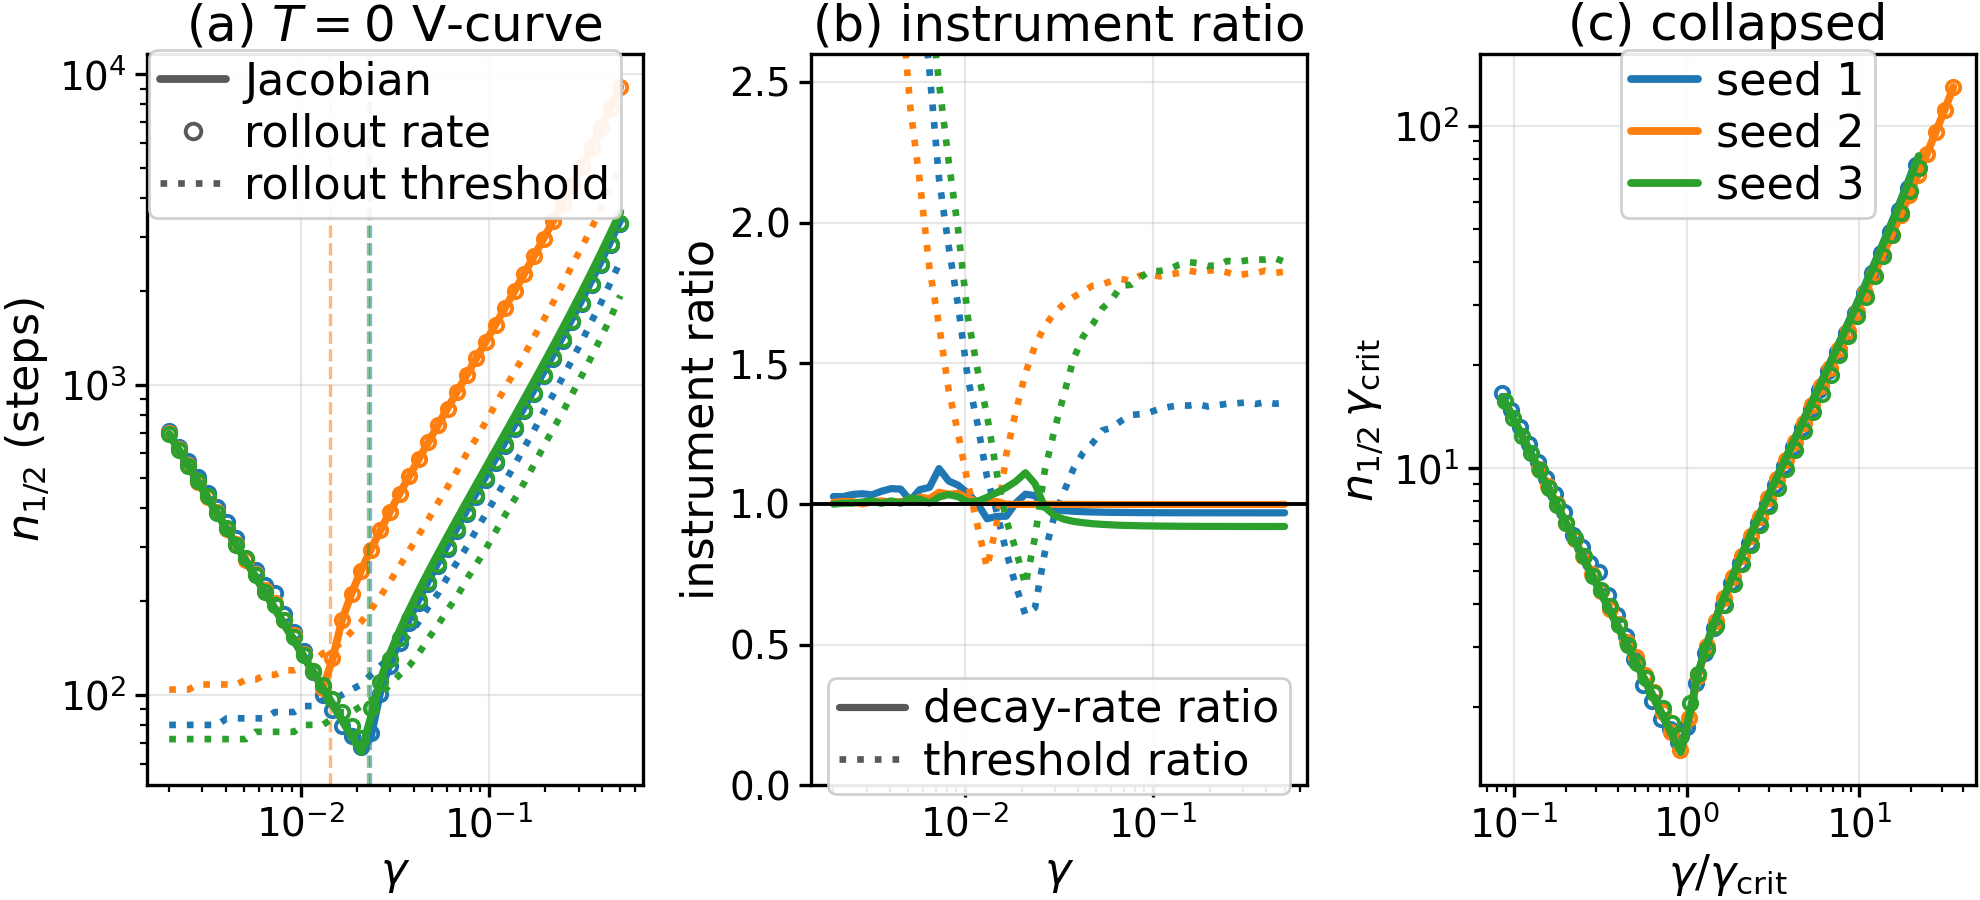
\includegraphics[width=0.90\linewidth]{figs/fig2_two_instruments.png}
\caption{The V-curve measured a second way. (a) $T=0$ $n_{1/2}(\gamma)$ per emergent seed on the one-step Jacobian (I-J, lines), the rollout envelope-rate instrument (I-R3, circles) and the rollout first-crossing threshold (I-R1, dotted), at $\delta=0.05$ rad. (b) The per-$\gamma$ instrument ratio: the rate ratio sits on $1$, the threshold ratio is offset and flat in $\gamma$ above $\gamma_{\rm crit}$. (c) The same data in collapsed variables. \emph{(Emergent MLP, 3 seeds, dim 4, hidden 64, $\varepsilon=0.05$, float64, $T=0$, pre-registered $\Rightarrow$ evidence.)}}
\end{figure}

\section{The friction-hole vault, on both arms}\label{app:vault}

\emph{Designed $SO(2)$ plus an analytic field, 3 seeds $\Rightarrow$ verification; emergent MLP, 3 seeds $\Rightarrow$ evidence. Pre-registered on both arms. All cells \texttt{langevin\_noise="fdt"}, Newtonian kinetic mode, $\Delta=0.5$ rad.}

\emph{Mechanism.} The shipped field is absorb-only, $p\leftarrow(1-\gamma_\phi)(1-\gamma)p+\sigma(\gamma)\xi$ with $\sigma^2=MT\gamma(2-\gamma)$ set by the \emph{scalar} $\gamma$, so with $\gamma_{\rm eff}=1-(1-\gamma)(1-\gamma_\phi)$, $T_{\rm local}=T\gamma(2-\gamma)/[\gamma_{\rm eff}(2-\gamma_{\rm eff})]$ and $D_\theta=\varepsilon T\gamma(2-\gamma)/(2F^2\gamma_{\rm eff}^2)$: a vault of $(\gamma_{\rm eff}/\gamma)^2$. A coupled bath would give $D_\theta\propto\gamma_{\rm eff}^{-1}$ and a vault of $[\gamma_{\rm eff}(2-\gamma)]/[\gamma(2-\gamma_{\rm eff})]=13.88\times$ at $\gamma=0.05$, $\gamma_\phi=0.5$. The hypotheses differ by $7.942\times$; the coupled-bath value is a refuted prediction and never the vault.

\emph{Designed arm.} $\mathrm{Var}(p_i)/(M_iT)=0.9986$ ($\gamma_\phi=0$), $0.36171\pm0.00129$ ($0.1$), $0.23044$ ($0.2$), $0.17513$ ($0.3$), $0.12600\pm0.00031$ ($0.5$; absorb prediction $0.12591$), so $T_{\rm local}=1.26\times10^{-4}$, a $7.94\times$ refrigerator. $\mathrm{MSD}/\text{pred}_{\rm absorb}=1.0011\pm0.0215$ over 15 cells; the $D_\theta$-based vault is $8.42\times$, $22.39\times$, $44.31\times$, $107.77\pm4.78\times$ at $\gamma_\phi=0.1/0.2/0.3/0.5$ (absorb prediction $110.25$). The direct first-passage vault reads $86.97\pm2.94\times$ and is boundary-layer biased on the outside arm ($\ell_\theta/\Delta=0.079$), so $107.77\times$ is the quoted number and travels with its estimator's name. Scalar control at the same $\gamma_{\rm eff}$: $13.28\pm0.12\times$ with $\mathrm{Var}(p)=M_iT$ intact, field/scalar $8.11\pm0.37$ against a predicted $7.942$. At $T=0$ the hole erases nothing (drift $\le1.75\times10^{-12}$ rad per 200k steps inside and outside, 12/12 cells; $\big||\lambda|_{\max}-1\big|\le2.0\times10^{-15}$ over 27 cells including the hole edge) and attenuates the \emph{write} instead: $\theta_{\rm settle}({\rm in})/\theta_{\rm settle}({\rm out})=0.09576$ against the transport law's $0.095238$.

\emph{Emergent arm.} The coset there is a bounded mode ($\mu^2_{\rm adiab}=2.77\times10^{-2}$--$8.93\times10^{-2}$), so the designed block estimator is biased low by up to $55\%$ and is replaced by a window-free Ornstein--Uhlenbeck fit $\mathrm{MSD}(n)=A(1-e^{-n/\tau})$, $\hat D=A/(2\varepsilon\tau)$, cross-validated on designed before use ($112.58\pm1.09\times$ against the banked $107.77\pm4.78\times$; $14.16\pm1.38\times$ against $13.28\pm0.12\times$; $8.03\pm0.80$ against $8.11\pm0.37$).

\begin{table}[!htb]\centering\scriptsize
\caption{The refrigerator law transfers exactly to an emergent register: $\mathrm{Var}(p_i)/(M_iT)$ against the absorb-only prediction, 2048 walkers $\times$ 40 samples, 3 emergent seeds; over all 24 field cells observed/absorb $=0.9998\pm0.0019$, and at $\gamma_\phi=0.5$ $T_{\rm local}/T=0.12570$, a $7.955\times$ refrigerator against $7.942$ predicted. The coupled bath predicts $1.0$ everywhere and is measured at $0.2235$.}
\begin{tabular}{lcccccc}
\toprule
$T$ & $\gamma_\phi$ & $\gamma_{\rm eff}$ & absorb pred. & coupled pred. & measured & obs/absorb\\
\midrule
$4\times10^{-3}$ & $0.0$ & $0.050$ & $1.00000$ & $1.0$ & $0.99815\pm0.00257$ & $0.9981$\\
$4\times10^{-3}$ & $0.1$ & $0.145$ & $0.36249$ & $1.0$ & $0.36326\pm0.00067$ & $1.0021$\\
$4\times10^{-3}$ & $0.2$ & $0.240$ & $0.23082$ & $1.0$ & $0.23062\pm0.00080$ & $0.9991$\\
$4\times10^{-3}$ & $0.3$ & $0.335$ & $0.17480$ & $1.0$ & $0.17473\pm0.00046$ & $0.9996$\\
$4\times10^{-3}$ & $0.5$ & $0.525$ & $0.12591$ & $1.0$ & $0.12592\pm0.00055$ & $1.0001$\\
$8\times10^{-3}$ & $0.5$ & $0.525$ & $0.12591$ & $1.0$ & $0.12548\pm0.00032$ & $0.9966$\\
\bottomrule
\end{tabular}
\end{table}

\begin{table}[!htb]\centering\scriptsize
\caption{The hole confines an emergent register, and the laundering control shows friction alone does not. $T=4\times10^{-3}$, 1024 walkers, burn-in $20\,000$--$80\,000$ steps, spread by interquartile range; ``hop'' means $|\theta|>1$ rad. The pre-registered stationary-spread comparison is \emph{void} here and no in/out spread ratio may be quoted from these checkpoints: the control that must return exactly $1.000$ returns $0.4586\pm0.1181$.}
\begin{tabular}{llccccc}
\toprule
seed & arm & $\gamma_{\rm eff}$ & $\sigma_\theta$ (IQR) & hop fraction & Boltzmann at $T_{\rm local}$ & obs/pred\\
\midrule
42 & no hole, $\gamma=0.05$ & $0.050$ & $0.40795$ & $5.50\%$ & $0.24073$ & $1.6946$\\
42 & scalar $0.525$ (control) & $0.525$ & $0.20034$ & $0.73\%$ & $0.24073$ & $0.8322$\\
42 & $\gamma_\phi$ hole & $0.525$ & $0.06442$ & $0.0000$ & $0.08542$ & $0.7542$\\
43 & no hole & $0.050$ & $1.17601$ & $42.97\%$ & $0.46059$ & $2.5533$\\
43 & scalar $0.525$ & $0.525$ & $0.35335$ & $10.20\%$ & $0.46059$ & $0.7672$\\
43 & $\gamma_\phi$ hole & $0.525$ & $0.08628$ & $0.0000$ & $0.16343$ & $0.5279$\\
44 & no hole & $0.050$ & $0.36922$ & $2.36\%$ & $0.24034$ & $1.5363$\\
44 & scalar $0.525$ & $0.525$ & $0.21574$ & $0.26\%$ & $0.24034$ & $0.8977$\\
44 & $\gamma_\phi$ hole & $0.525$ & $0.07279$ & $0.0000$ & $0.08528$ & $0.8535$\\
\bottomrule
\end{tabular}
\end{table}

\emph{The diffusion law on the emergent arm.} On bounded cells, $\hat D_{\rm ou}/D_{\rm absorb}=1.0480$ ($\gamma_\phi=0$, 1 cell), $1.1026\pm0.0799$ ($0.1$, 4), $1.0158\pm0.0519$ ($0.2$, 5), $1.0552\pm0.0496$ ($0.3$, 5), $1.0418\pm0.0519$ ($0.5$, 6); against the coupled bath the same cells give $0.1312\pm0.0065$ at $\gamma_\phi=0.5$. Law-referenced vault $106.1\pm5.0\times$ (6 cells; prediction $110.25\times$; designed $107.77\pm4.78\times$). A measured/measured ratio over the same cells reads $297.8\pm196.8\times$ (median $234.4\times$); it is recorded and is never the vault number, because 5 of the 6 $\gamma_\phi=0$ cells fail the bounded test ($\sigma^{\rm ou}_\theta=0.42$--$885$ rad against a Boltzmann $0.24$--$0.65$), while every $\gamma_\phi\ge0.2$ cell passes.

\emph{The contrast number is designed-only, and the failure mode is the control.} A scalar $\gamma$ does not cool --- $\mathrm{Var}(p)/(MT)=0.99288\pm0.02354$ at $\gamma=0.525$ with no field, where both hypotheses predict $1.0$, against $0.126$ for the field at the same $\gamma_{\rm eff}$ --- so the mechanism statement (a friction field is not locally stronger friction; it is locally stronger friction \emph{plus} a local refrigerator) stands on emergent. The contrast measures $23.39\pm10.06$ (per-cell $9.14/25.75/26.96/21.70/41.31/15.48$) against a pre-registered band $[6.5,9.5]$ and a falsifier at $>14$: it fired. The cause is the control arm, whose own $\hat D_{\rm ou}/D_{\rm flat}$ is $1.1768/3.7319/3.3782/2.7999/5.2284/2.0506$ --- at $\gamma=0.525$ with no cooling the emergent coset is still anharmonically delocalised --- while the field arm sits on the absorb law at $1.02$--$1.15$. The \emph{direction} transfers; the \emph{number} $8.11\pm0.37$ is a designed quantity.

\emph{First passage, and the confound it exposed.} An emergent potential has no rotational symmetry, so a $\theta=\pi$ ``outside'' arm is not a vacuum: $|\nabla V|=0.0420/0.1049/0.0414$ there against $0.0000$ at $\theta=0$, $V(\pi)-V(0)=+0.03163/+0.06003/+0.04315$, and $\mu^2_{\rm adiab}$ differing by up to $2.15\times$ between the sites. Any emergent first-passage number quoted against a $\theta=\pi$ baseline is confounded and a same-site baseline is required. Same-site vaults ($|\Delta\theta|\ge0.5$ rad, $T=4\times10^{-3}$, $\gamma=0.05$, 256 walkers, hole radius $1.0$): $>1379\times$ (seed 42), $35.5\times$ (43), $>1290\times$ (44), the first and third being censoring-limited \emph{lower bounds} ($86.7\%$ and $93.4\%$ censored at a $10^6$-step cap; closing them needs $\approx10^7$ steps per walker). The pre-registered $>300\times$ holds 2/3 and the falsifier fires on seed 43, already flagged as geometrically atypical --- softest $\mu^2$, shallowest barrier ($6.8\times10^{-3}$), coset at $\sigma_\theta/\Delta=0.92$ outside and $0.33$ inside, never leaving the diffusive regime. The confound's signature is seed 44, whose $\theta=\pi$ first passage ($15585$) is $20\times$ its own $\theta=0$ value ($775$) and whose scalar control reads $0.27\times$: more friction apparently \emph{speeding} escape, impossible for a stationary register.

\emph{Scope carried by the whole emergent arm.} Three model seeds; a single PRNG stream per cell, so every spread is across model seeds, not noise realizations; both temperatures above $T^\star$ while the designed study's trustworthy-cell restriction is $T\le3\times10^{-3}$, so every measurement is squeezed between $T^\star$ and delocalisation and only cells passing the bounded test support a law claim. The hole is a ball of radius $1.0$ in the full 4-D space, so excursions of order $1.0$ ($\approx4.5\sigma_r$) leave it --- a plausible contributor to seed 43's low vault, not separately measured. No temperature field was built.

\begin{figure}[!htb]
\centering
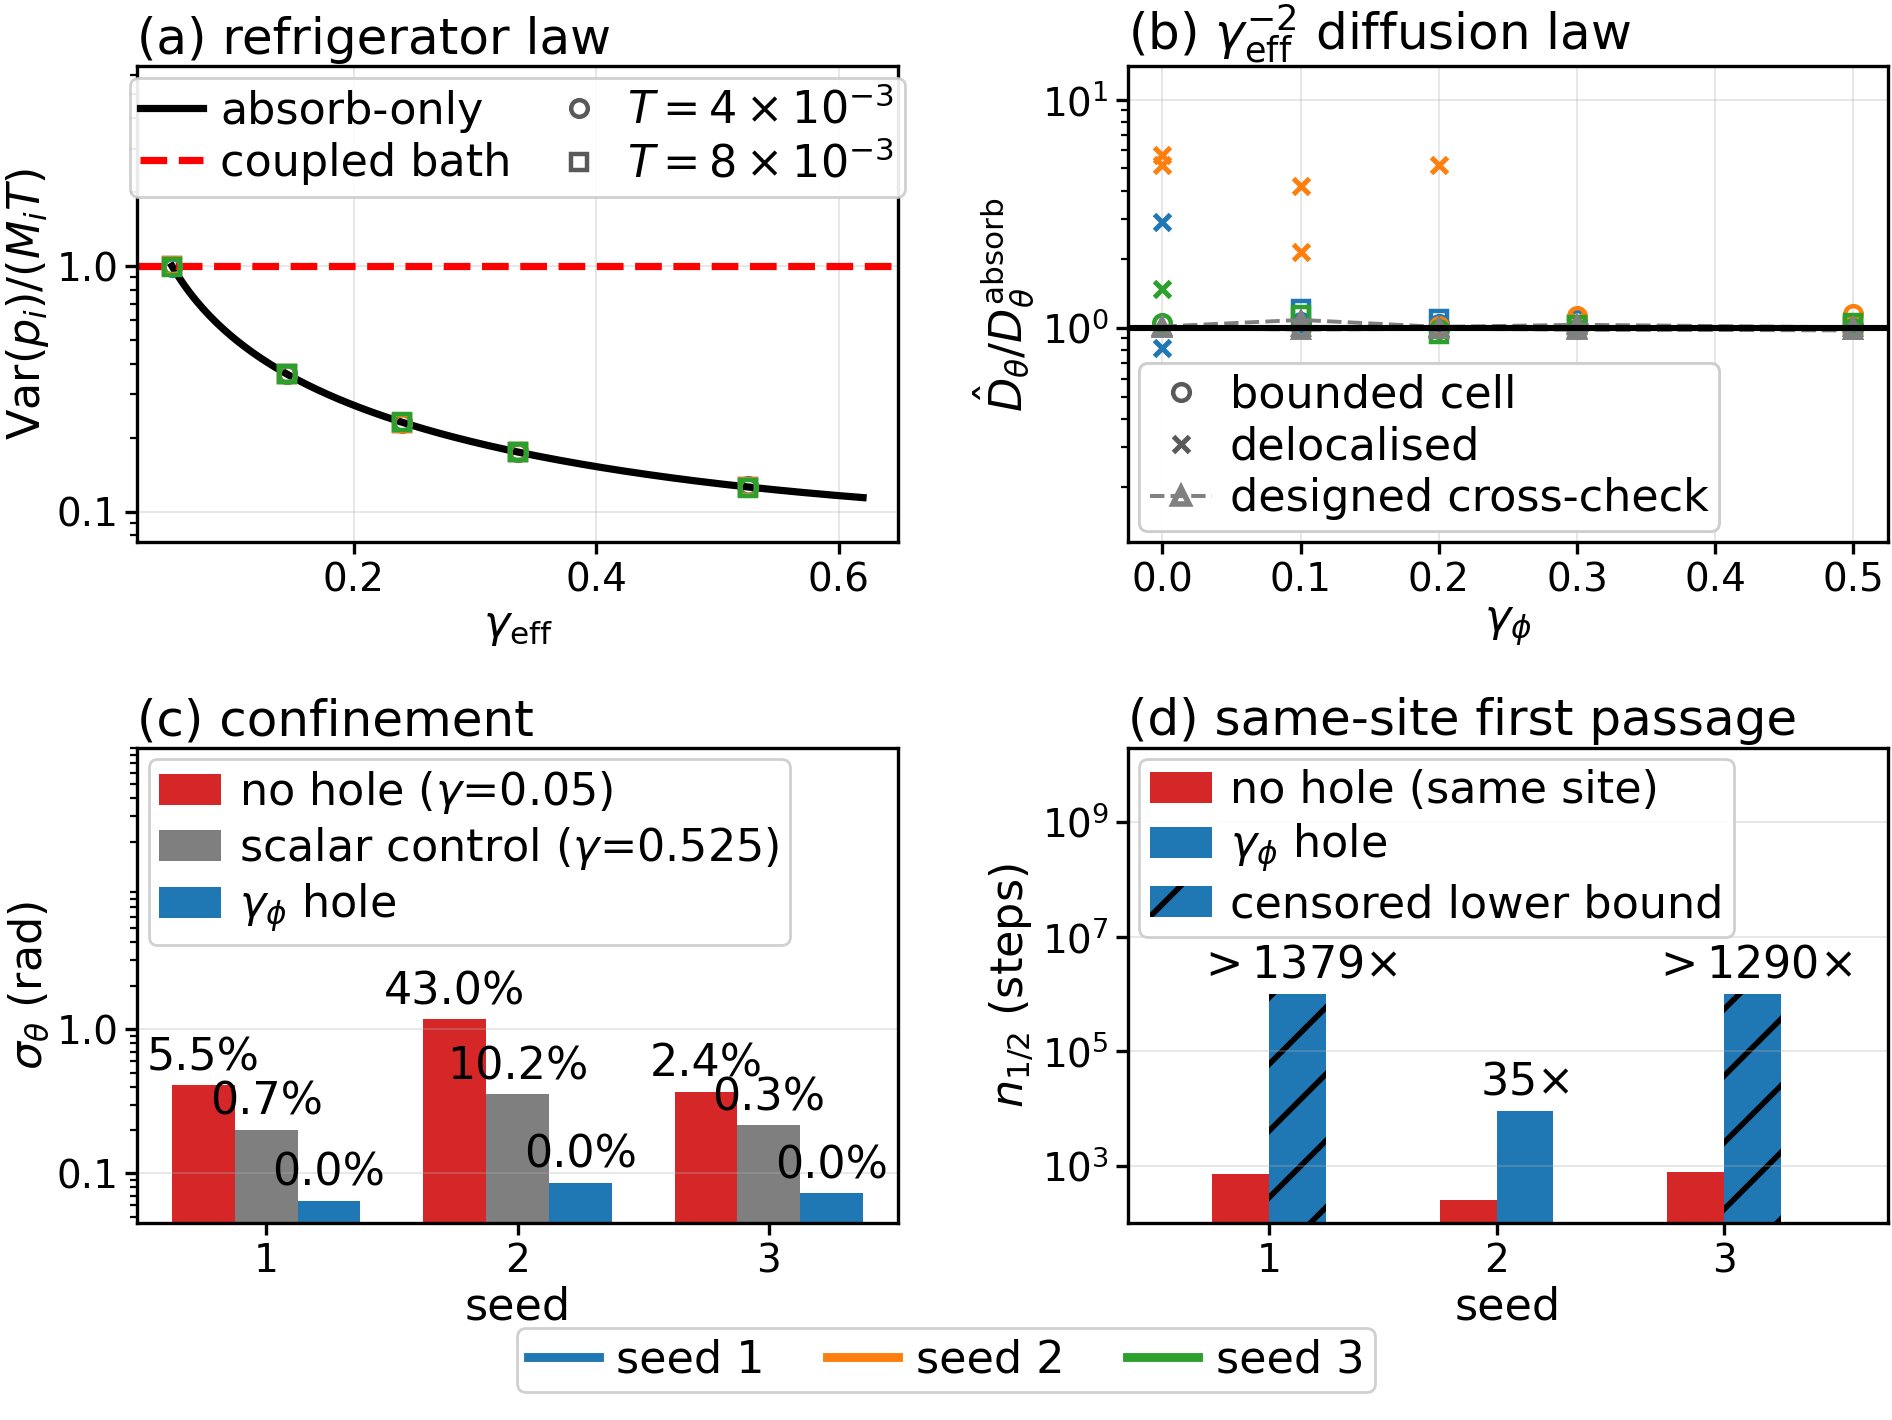
\includegraphics[width=0.86\linewidth]{figs/figC2_vault_emergent.png}
\caption{The vault on an emergent register; panels are labelled by the pre-registered prediction each tests. (a) The refrigerator law, $\mathrm{Var}(p_i)/(M_iT)$ against $\gamma_{\rm eff}$ for 3 seeds $\times$ 2 temperatures, on the absorb-only curve with the coupled-bath prediction (dashed) rejected. (b) The $\gamma_{\rm eff}^{-2}$ diffusion law: bounded cells as circles and squares, delocalised cells as crosses, the designed cross-check overlaid. (c) Confinement: stationary spread and hop fraction for no hole, the scalar control and the hole. (d) Same-site first passage; hatched bars are censored lower bounds. \emph{(Emergent MLP, 3 seeds, $T\in\{4,8\}\times10^{-3}$, both above $T^\star$, $\Delta=0.5$ rad $\Rightarrow$ evidence.)}}
\end{figure}

\section{Exact store-level deletion: prior art and the measured tables}\label{app:deletion}

\emph{Designed atom store, dim 3, capacity 8--64, no learning anywhere $\Rightarrow$ verification of the mechanism's exactness. Every deletion statement carries its scope: store level only, under the three stated conditions, with recency-based eviction permanently excluded.}

\emph{Prior art, in full.} Uniquely represented (canonical) data structures date to Snyder (1977) and Andersson \& Ottmann (1995); \emph{obliviousness}, a distributional condition on the memory representation which explicitly does not require canonical representation, is Micciancio's (1997); the weak and strong history-independence notions used here are Naor \& Teague's (2001); the open-addressed realisation is Blelloch \& Golovin's (2007), whose table is a stable matching between keys and slots under a global key priority, and it is that priority-greedy rule and that delete-time fix-up cascade we use; Blelloch, Golovin \& Vassilevska (2008) had already taken unique representation into computational geometry. We claim no priority over order-independent placement and no novelty for the displacement rule or its delete-time repair. New is the composition: slots that are a lattice packing, so the canonical representation carries a minimum-separation certificate; content that is a continuously decaying amplitude whose decay commutes with deletion; a canonical object that is an energy function a dynamical read relaxes into; and a price that is negative where strong history independence is known to cost as much as an exponential slowdown relative to the weak notion for comparison-based structures (Buchbinder \& Petrank, 2003). ``Fix-up cascade'' is our name for the \texttt{NEXT}-chain delete-time repair of their Figure 1; the algorithm is theirs either way.

\emph{Exactness, measured at zero tolerance.} 24 exhaustive orders at $n=4$, 200 random orders at $n\in\{8,16,40,64\}$, 100 write/delete interleavings and mid-decay deletes: all bit-identical, minimum spacing exactly $1.540000$; on the shipped store the centres, payloads, amplitudes and active mask are byte-equal and $V(q)$ is byte-equal on 64 random queries. \emph{The packing price is negative:} at $K=64$ the canonical rule admits $61/64$ offered keys deterministically ($\sigma=0$), per-offered $0.9531$, rising to $64/64$ when the sizing is inflated by $\times1.05$, where the stochastic refuse-and-relocate allocator admits $43/64$ on the same seeds (per-offered $0.6719$); delete-time churn is $2.836$ moves per delete at full load. \emph{At overflow, without the waitlist, exactness fails:} with 7 cells and 8 offers, $\mathrm{AUC}(n_{\rm live})=1.00000\pm0.0000$, white-box address-depth $\mathrm{AUC}=0.91409\pm0.0813$, byte-equal fraction $0.0000$. A pre-registration that failed informatively: $\mathrm{AUC}(z_{\rm hole})\ge0.85$ was registered there and measured $0.576$, because the fix-up cascade \emph{fills} the freed cell with a re-placed survivor.

\begin{table}[!htb]\centering\scriptsize
\caption{The laundering control that fires. Designed store, shipped two-phase read, no learning anywhere; 8 targets $\times$ 3 seeds, 128 paired worlds per target, 18 amplitude levels. Against an \emph{exact} adversary a boolean TTL flag inside the same store is as detectable as an $e^{-\lambda t}$ amplitude, so there is no measurable differentiator at the AUC level; the control fails to fire only against a resolution-limited adversary, and that resolution is our own modelling choice --- which is why the main text leads with the retrieval geometry instead.}
\begin{tabular}{lccc}
\toprule
adversary & physical decay & TTL flag in the same store & separation\\
\midrule
white-box, exact & $1.000$ & $1.000$ & $0.000$\\
query-level membership, exact & $0.983$ & $1.000$ & $0.017$\\
query-level membership, $\sigma_{\rm obs}=0.1$ & $0.559$ & $0.996$ & $0.437$\\
\bottomrule
\end{tabular}
\end{table}

\emph{What decays and what does not.} Against an exact adversary the white-box per-example AUC is $1.000$ at all 18 amplitude levels down to the floor; what decays is the effect size, the depth gap being $0.3935\cdot A$ to four decimals at every level (the pre-registered closed form $1-e^{-1/2}$) and $d'$ falling $1\,560\to79.6$, exactly linear in $A$ --- the pre-registered falsifier fired on the AUC metric, as registered. Against a resolution-limited adversary the grading is real and the pre-registered law survives, $A_{75}=2.57\sigma_{\rm obs}$ measuring $0.0780/0.2627/0.7537$ at $\sigma_{\rm obs}=0.03/0.1/0.3$ against predicted $0.0771/0.2570/0.7710$; but $\sigma_{\rm obs}$ is our modelling choice, so its defensible use is mechanistic, never protective. \emph{State the $|c|$ distribution with any retention number:} every retention magnitude here is for the controller-placed disk (proposal radius $2.2869$, packing bound $8.00$); on a max-radius ring the same store gives retention $0.500$ at $A=0.06$ where this placement gives $0.886$. \emph{Retrieval geometry:} $R_{50}$ contracts $1.146/1.083/0.979/0.874/0.752$ as $A:1\to0.5\to0.2\to0.1\to0.06$, matching the pre-registered saddle prediction at all five points ($\pm0.20$), where a TTL vector store's lookup radius is a constant hard step at $0.75$--$0.77$.

\emph{The trilemma, and what it costs.} The shipped store drops amplitude-independent address hold, which is why effective lifetime correlates $r=-0.85$ with $a_i^2$; the recommended gated-stiffness channel drops amplitude-independent latency and is the compute-adaptive-read dial --- and it is \emph{not} the shipped arm. Both previously proposed repairs are refuted: multiplying payloads by amplitudes kills the value criterion at $A=1-\text{tol}/|a_i|$ (measured death amplitudes $0.90/0.80/0.70/0.30$ against the formula's $0.900/0.860/0.767/0.300$) and inverts the payload dependence; launching the payload coordinate at the address-mapped point breaks the anti-decoration guard, after which a trivial substitute passes $0.672$ of queries with no dynamics at all. Behind its flag the gated channel contracts $R_{50}$ $1.135\to0.771$, retention std $0.274\to0.016$, worst codeword $0.398\to0.972$; the registered payload-independence test \emph{fails as a correlation} ($|r|$ only $0.846\to0.667$) and passes as an effect size; and at $\gamma_{\rm read}=0$ it is oscillatory, period $2\pi/\sqrt{\kappa(g_0+A)}$ (log-log slope $-0.5264$), so no settling law may be quoted without a nonzero read friction. \emph{No deletion-cost statement is made:} the shipped canonical synchronisation is an $O(n)$ rebuild per operation and the amortized-cost experiment has not been run.

\section{Prominent negatives}\label{app:negatives}

\emph{Every negative below is on the record with its measurement; none is dropped, and each anchors a future-work item.}

{\tiny\begin{center}
\begin{tabular}{p{0.28\linewidth}p{0.66\linewidth}}
\toprule
claim tested & result\\
\midrule
A continuous coset register emerges from training & No: an MLP potential on symmetric data yields a mid-spectrum massive mode ($1.7$--$4.9\times$ softer than the stiffest), capacity $\approx1$--$1.6$ bits, complete relaxation of any written value. The $T=0$ latch is designed-only.\\
Raw $T/\gamma$-exponents discriminate designed from emergent & No: a matched designed control reproduces the same shallow slopes; only $\ell_\theta/\Delta$-controlled cells and $|\lambda_{\rm coset}|$ discriminate. Never an $n_{1/2}$ without $\Delta$ and $\ell_\theta/\Delta$.\\
The friction hole thermalizes locally (coupled bath) & Rejected by a pre-registered measurement, by a factor $8.11$: the field is absorb-only and the vault is $107.77\pm4.78\times$, against $13.28\pm0.12\times$ for the scalar control.\\
A friction field can \emph{forget} a coset & No: at $T>0$ it \emph{lengthens} coset memory. Erasing latched content needs a temperature or tilt field --- which explains the observed failure of a learned friction field to recover fit on a stationary vacuum.\\
Our own sign-flip prediction, in both observables & Falsified in one: a register written at the washboard minimum cannot flip back, and both signs coexist on one checkpoint for different observables. A sign-flip figure that does not name the initial condition is meaningless.\\
Amplitude decay reduces an exact adversary's distinguishability & No, at any point in an item's life: white-box AUC $1.000$ at all 18 amplitude levels; what decays is the effect size. The graded curve exists only relative to a stated adversary resolution, our own modelling choice.\\
Canonical placement is exact at overflow without the waitlist & No: $\mathrm{AUC}(n_{\rm live})=1.000$, byte-equal fraction $0.0000$. Every deletion sentence carries its scope clause; recency eviction is permanently excluded.\\
The placement algorithm is ours & No: Blelloch \& Golovin (2007) own it outright, and unique representation in a geometric setting is also taken (2008). Our claim is the composition only.\\
A per-deletion cost claim can be made & No: the shipped synchronisation is an $O(n)$ rebuild per operation, so the amortized-cost formalism cannot be instantiated on our own code until that experiment runs.\\
The payload-lifetime coupling has a repair & Both proposed repairs are refuted, and the registered payload-independence statistic fails as a correlation while passing as an effect size. At zero read friction the gated channel is oscillatory, not relaxational.\\
\bottomrule
\end{tabular}

\end{center}
\begin{center}
\begin{tabular}{p{0.28\linewidth}p{0.66\linewidth}}
\toprule
claim tested & result\\
\midrule
A pseudo-Goldstone tilt is a lifetime dial on a learned store & Refuted \emph{in sign}: a tilt monotonically \emph{reduces} the smallest eigenvalue on two independent implementations and every family, because a written site is not a common vacuum of its own atoms. The relation survives only in the single-atom geometry it was specified in.\\
A tilt sets the soft scale on a learned store & No: the confinement floors the soft eigenvalue at $2\alpha$, capping lifetime at $\tau_{\max}=\Gamma/2\alpha$. The registered damped-mode floor is confirmed, the $1/\text{tilt}$ branch unreachable, and lowering the confinement breaks the write.\\
The lifecycle's protected-fraction leg is exercised & No: 0 refusals on the stream at the measured operating point. Reported as \emph{unexercised} --- not working and not broken.\\
A task-level payoff is claimed & No: forgetting here is shown predictable, controllable, removable and schedulable, not shown to improve a downstream metric. External benchmarks won on their own headline metric = ZERO.\\
The field/scalar vault contrast transfers to an emergent register & No: $23.39\pm10.06$ against $8.03\pm0.80$ from the identical estimator on designed; the pre-registered falsifier fired. The cause is the laundering control itself, off its own law by $1.18$--$5.23\times$. The number is designed-only; its direction transfers.\\
The emergent stationary-spread diagnostic is measurable above $T^\star$ & No: its own control, which must return $1.000$, returns $0.4586\pm0.1181$ --- the no-hole arm is a hopping rotor, so no in/out spread ratio may be quoted. The confinement statement replaces it.\\
A $\theta=\pi$ baseline is valid for emergent first passage & No: $|\nabla V|=0.042$--$0.105$ there against $0.0000$ at $\theta=0$, and one seed's scalar control reads $0.27\times$, i.e.\ more friction apparently speeding escape. Same-site baselines are required; the designed arm is protected by symmetry but was never checked, and that check is owed.\\
Threshold instruments are usable below $\gamma_{\rm crit}$ & No: a first-crossing $n_{1/2}$ puts its argmin at the grid edge with a below-slope of $+0.0623\pm0.0120$ where the law says $-1$, and last-crossing carries an additive half-period bias. Only the envelope-rate instrument is quotable there.\\
Our microscopic explanation of the instrument offset & Wrong, though the offset itself is real, constant and quotable: the pre-registered single-slow-mode projection fails (amplitude fraction $0.638/0.644/0.327$ does not order like the angular overlaps) and the early-window ratio $0.52$--$0.85$ is amplitude-independent --- multi-mode transient, not anharmonicity.\\
The emergent first-passage vault is measured & Only bounded: $>1379\times$ and $>1290\times$ at $86.7\%$/$93.4\%$ censoring, and $35.5\times$ on the geometrically atypical seed. Three seeds cannot say which is typical.\\\\
\bottomrule
\end{tabular}
\end{center}\par}

\emph{Anonymization note.} Any supplementary or linked material, including code, is anonymized; only an anonymized snapshot may be linked.


\end{document}
